\documentclass[11pt, a4paper]{article}

% Fonts and Encoding
\usepackage[utf8]{inputenc}
\usepackage[T1]{fontenc}
\usepackage{lmodern}

% Math and Symbols
\usepackage{amsmath, amssymb, amsthm, amsfonts, mathrsfs, mathtools}

% Layout and Geometry
\usepackage{geometry}
\geometry{a4paper, margin=1in}

% Formatting and Graphics
\usepackage{graphicx, xcolor, enumitem, booktabs, array, tabularx}

% TikZ for Illustrations
\usepackage{tikz}
\usetikzlibrary{arrows.meta, positioning, shapes.geometric, calc, backgrounds, matrix}

% Clickable Links and TOC
\usepackage{hyperref}
\hypersetup{
    colorlinks=true,
    linkcolor=blue,
    filecolor=magenta,      
    urlcolor=cyan,
    pdftitle={Advanced Mathematics Topic},
}

% Theorem Environments
\newtheorem{theorem}{Theorem}[section]
\newtheorem{lemma}[theorem]{Lemma}
\newtheorem{proposition}[theorem]{Proposition}
\newtheorem{corollary}[theorem]{Corollary}
\theoremstyle{definition}
\newtheorem{definition}{Definition}[section]
\newtheorem{axiom}{Axiom}[section]
\newtheorem{example}{Example}[section]
\theoremstyle{remark}
\newtheorem{remark}{Remark}[section]

% Custom Commands (Enforced standard notation)
\newcommand{\R}{\mathbb{R}}
\newcommand{\N}{\mathbb{N}}
\newcommand{\Z}{\mathbb{Z}}
\newcommand{\Q}{\mathbb{Q}}
\newcommand{\E}{\mathbb{E}}
\newcommand{\Prob}{\mathbb{P}}
\newcommand{\F}{\mathcal{F}}

\begin{document}

\title{\textbf{Advanced Abstract Mathematics: The Integers Modulo $n$}\\ \Large Rigorous Foundations and Applications in Quantitative Modeling}
\author{Tashfeen Omran}
\date{\today}
\maketitle

\tableofcontents
\newpage

\section{Comprehensive Introduction, Context, and Prerequisites}

\subsection{Historical Context and Motivation}
The formalization of modular arithmetic marks a watershed moment in the history of abstract algebra and number theory. Introduced systematically by Carl Friedrich Gauss in his seminal 1801 work, \textit{Disquisitiones Arithmeticae}, the concept of congruence provided a rigorous framework for solving Diophantine equations and understanding the periodic nature of integers. Historically, mathematicians grappled with the concept of "clock arithmetic"—where numbers wrap around after reaching a certain value—but lacked the set-theoretic machinery to treat these wrapped values as distinct mathematical objects. By defining equivalence relations and their corresponding equivalence classes, modern mathematics successfully abstracted the integers into finite quotient rings, laying the groundwork for modern cryptography, coding theory, and stochastic simulations.

\subsection{Core Concepts and Axioms}
The study of the integers modulo $n$, denoted as $\Z_n$, is fundamentally an exploration of quotient structures. We begin with the standard ring of integers, $\Z$, and impose an equivalence relation based on divisibility.

\begin{definition}[Congruence Modulo $n$]
Let $n \in \Z$ such that $n \ge 2$. For $a, b \in \Z$, we say that $a$ is congruent to $b$ modulo $n$, written as $a \equiv b \pmod n$, if and only if $n \mid (a - b)$. Equivalently, there exists an integer $k \in \Z$ such that $a - b = kn$.
\end{definition}

This relation is an equivalence relation (reflexive, symmetric, and transitive). Consequently, it partitions the set of integers into $n$ disjoint equivalence classes, called \textit{residue classes}.

\begin{definition}[Equivalence Class]
The equivalence class of an integer $a$ modulo $n$, denoted by $[a]$, is the set of all integers congruent to $a$ modulo $n$:
\[
[a] = \{ x \in \Z : x \equiv a \pmod n \} = \{ a + kn : k \in \Z \}
\]
\end{definition}

The set of all such distinct equivalence classes is denoted by $\Z_n = \{[0], [1], \dots, [n-1]\}$. 

\subsection{Intuition and Set-Theoretic Foundations}
Intuitively, $\Z_n$ can be visualized as a mapping from the infinite, linear number line $\Z$ onto a finite, circular space. Every integer is dropped into one of $n$ "buckets" based on its remainder when divided by $n$ (via the Division Algorithm). The profound leap in abstract algebra is treating these buckets (which are infinite sets themselves) as single elements in a new algebraic structure. We define operations on these sets:
\[
[a] + [b] = [a + b] \quad \text{and} \quad [a] \cdot [b] = [a \cdot b]
\]
The critical logical hurdle is proving that these operations are \textit{well-defined}. Because $[a]$ can be represented by any element within its set (e.g., $[2] = [7]$ in $\Z_5$), we must guarantee that choosing different representatives does not change the resulting equivalence class of the sum or product.

\subsection{Key Theorems and Prerequisites}
\begin{theorem}[Well-Defined Operations in $\Z_n$]
Addition and multiplication in $\Z_n$ are well-defined. If $[a] = [c]$ and $[b] = [d]$ in $\Z_n$, then $[a + b] = [c + d]$ and $[a \cdot b] = [c \cdot d]$.
\end{theorem}

\textbf{Prerequisites for this Chapter:}
\begin{itemize}
    \item \textbf{Set Theory:} Understanding partitions, disjoint sets, and Cartesian products.
    \item \textbf{Equivalence Relations:} Mastery of reflexivity, symmetry, and transitivity.
    \item \textbf{Number Theory:} The Division Algorithm ($a = qn + r$) and the definition of divisibility ($a \mid b$).
    \item \textbf{Proof Techniques:} Direct proof, proof by contradiction, and algebraic manipulation of integer equations.
\end{itemize}

\newpage
\section{Detailed Homework Solutions}

\subsection{Exercise 9.54}
\textbf{Problem:} Construct the addition and multiplication tables for $\Z_4$ and $\Z_5$.

\textbf{Solution:}
We compute the sums and products modulo $n$ for each pair of elements. For $\Z_4$, the elements are $\{[0], [1], [2], [3]\}$. For $\Z_5$, the elements are $\{[0], [1], [2], [3], [4]\}$.

\renewcommand{\arraystretch}{1.5}
\begin{table}[h]
\centering
\begin{tabular}{>{$\displaystyle}c<{$} >{$\displaystyle}c<{$} >{$\displaystyle}c<{$} >{$\displaystyle}c<{$} >{$\displaystyle}c<{$}}
\toprule
+ & [0] & [1] & [2] & [3] \\
\midrule
{[0]} & [0] & [1] & [2] & [3] \\
{[1]} & [1] & [2] & [3] & [0] \\
{[2]} & [2] & [3] & [0] & [1] \\
{[3]} & [3] & [0] & [1] & [2] \\
\bottomrule
\end{tabular}
\quad\quad
\begin{tabular}{>{$\displaystyle}c<{$} >{$\displaystyle}c<{$} >{$\displaystyle}c<{$} >{$\displaystyle}c<{$} >{$\displaystyle}c<{$}}
\toprule
\cdot & [0] & [1] & [2] & [3] \\
\midrule
{[0]} & [0] & [0] & [0] & [0] \\
{[1]} & [0] & [1] & [2] & [3] \\
{[2]} & [0] & [2] & [0] & [2] \\
{[3]} & [0] & [3] & [2] & [1] \\
\bottomrule
\end{tabular}
\caption{Addition and Multiplication Tables for $\Z_4$}
\end{table}

\renewcommand{\arraystretch}{1.5}
\begin{table}[h]
\centering
\begin{tabular}{>{$\displaystyle}c<{$} >{$\displaystyle}c<{$} >{$\displaystyle}c<{$} >{$\displaystyle}c<{$} >{$\displaystyle}c<{$} >{$\displaystyle}c<{$}}
\toprule
+ & [0] & [1] & [2] & [3] & [4] \\
\midrule
{[0]} & [0] & [1] & [2] & [3] & [4] \\
{[1]} & [1] & [2] & [3] & [4] & [0] \\
{[2]} & [2] & [3] & [4] & [0] & [1] \\
{[3]} & [3] & [4] & [0] & [1] & [2] \\
{[4]} & [4] & [0] & [1] & [2] & [3] \\
\bottomrule
\end{tabular}
\quad\quad
\begin{tabular}{>{$\displaystyle}c<{$} >{$\displaystyle}c<{$} >{$\displaystyle}c<{$} >{$\displaystyle}c<{$} >{$\displaystyle}c<{$} >{$\displaystyle}c<{$}}
\toprule
\cdot & [0] & [1] & [2] & [3] & [4] \\
\midrule
{[0]} & [0] & [0] & [0] & [0] & [0] \\
{[1]} & [0] & [1] & [2] & [3] & [4] \\
{[2]} & [0] & [2] & [4] & [1] & [3] \\
{[3]} & [0] & [3] & [1] & [4] & [2] \\
{[4]} & [0] & [4] & [3] & [2] & [1] \\
\bottomrule
\end{tabular}
\caption{Addition and Multiplication Tables for $\Z_5$}
\end{table}
\hfill $\blacksquare$

\subsection{Exercise 9.55}
\textbf{Problem:} In $\Z_8$, express the following sums and products as $[r]$, where $0 \le r < 8$.
(a) $[2] + [6]$ \quad (b) $[2] \cdot [6]$ \quad (c) $[-13] + [138]$ \quad (d) $[-13] \cdot [138]$

\textbf{Solution:}
We utilize the definitions $[a] + [b] = [a+b]$ and $[a] \cdot [b] = [ab]$, followed by the Division Algorithm to find the principal remainder $r$.
\begin{itemize}
    \item[(a)] $[2] + [6] = [8]$. Since $8 = 8(1) + 0$, we have $[8] = [0]$.
    \item[(b)] $[2] \cdot [6] = [12]$. Since $12 = 8(1) + 4$, we have $[12] = [4]$.
    \item[(c)] First, we reduce the operands modulo 8 to simplify computation. 
    $-13 = 8(-2) + 3 \implies [-13] = [3]$. 
    $138 = 8(17) + 2 \implies [138] = [2]$. 
    Therefore, $[-13] + [138] = [3] + [2] = [5]$.
    \item[(d)] Using the reduced forms from part (c), $[-13] \cdot [138] = [3] \cdot [2] = [6]$.
\end{itemize}
\hfill $\blacksquare$

\subsection{Exercise 9.56}
\textbf{Problem:} In $\Z_{11}$, express the following sums and products as $[r]$, where $0 \le r < 11$.
(a) $[7] + [5]$ \quad (b) $[7] \cdot [5]$ \quad (c) $[-82] + [207]$ \quad (d) $[-82] \cdot [207]$

\textbf{Solution:}
\begin{itemize}
    \item[(a)] $[7] + [5] = [12]$. Since $12 = 11(1) + 1$, we have $[12] = [1]$.
    \item[(b)] $[7] \cdot [5] = [35]$. Since $35 = 11(3) + 2$, we have $[35] = [2]$.
    \item[(c)] We reduce the operands modulo 11. 
    $-82 = 11(-8) + 6 \implies [-82] = [6]$. 
    $207 = 11(18) + 9 \implies [207] = [9]$. 
    Therefore, $[-82] + [207] = [6] + [9] = [15]$. Since $15 = 11(1) + 4$, we have $[15] = [4]$.
    \item[(d)] Using the reduced forms, $[-82] \cdot [207] = [6] \cdot [9] = [54]$. Since $54 = 11(4) + 10$, we have $[54] = [10]$.
\end{itemize}
\hfill $\blacksquare$

\subsection{Exercise 9.57}
\textbf{Problem:} Let $S = \Z$ and $T = \{4k : k \in \Z\}$. Thus, $T$ is a nonempty subset of $S$.
(a) Prove that $T$ is closed under addition and multiplication.
(b) If $a \in S - T$ and $b \in T$, is $ab \in T$?
(c) If $a \in S - T$ and $b \in T$, is $a+b \in T$?
(d) If $a, b \in S - T$, is it possible that $ab \in T$?
(e) If $a, b \in S - T$, is it possible that $a+b \in T$?

\textbf{Solution:}
\begin{itemize}
    \item[(a)] \textit{Proof of Closure:} Let $x, y \in T$. By definition, there exist integers $k_1, k_2 \in \Z$ such that $x = 4k_1$ and $y = 4k_2$. 
    For addition: $x + y = 4k_1 + 4k_2 = 4(k_1 + k_2)$. Since $k_1 + k_2 \in \Z$, $x + y \in T$.
    For multiplication: $x \cdot y = (4k_1)(4k_2) = 16k_1k_2 = 4(4k_1k_2)$. Since $4k_1k_2 \in \Z$, $x \cdot y \in T$. Thus, $T$ is closed under both operations.
    
    \item[(b)] \textit{Yes.} Let $a \in S - T$ and $b \in T$. Since $b \in T$, $b = 4k$ for some $k \in \Z$. Then $ab = a(4k) = 4(ak)$. Since $ak \in \Z$, $ab \in T$.
    
    \item[(c)] \textit{No.} We use a proof by contradiction. Suppose $a+b \in T$. Then $a+b = 4m$ for some $m \in \Z$. Since $b \in T$, $b = 4k$ for some $k \in \Z$. Substituting for $b$, we get $a + 4k = 4m$, which implies $a = 4m - 4k = 4(m - k)$. Since $m - k \in \Z$, this implies $a \in T$, which contradicts the premise that $a \in S - T$. Therefore, $a+b \notin T$.
    
    \item[(d)] \textit{Yes.} We provide a constructive example. Let $a = 2$ and $b = 2$. Neither $2$ nor $2$ is a multiple of $4$, so $a, b \in S - T$. However, $ab = 2 \cdot 2 = 4 = 4(1)$, which means $ab \in T$.
    
    \item[(e)] \textit{Yes.} We provide a constructive example. Let $a = 1$ and $b = 3$. Clearly, $1, 3 \in S - T$. However, $a + b = 1 + 3 = 4 = 4(1)$, which means $a+b \in T$.
\end{itemize}
\hfill $\blacksquare$

\subsection{Exercise 9.58}
\textbf{Problem:} Prove that the multiplication in $\Z_n, n \ge 2$, defined by $[a][b] = [ab]$ is well-defined.

\textbf{Solution:}
\textit{Proof (Direct):} To prove that multiplication is well-defined, we must show that if we choose different representatives for the equivalence classes, the resulting product's equivalence class remains unchanged. 
Let $[a] = [c]$ and $[b] = [d]$ in $\Z_n$. By definition of equivalence classes modulo $n$, this means $a \equiv c \pmod n$ and $b \equiv d \pmod n$. 
Therefore, there exist integers $k, j \in \Z$ such that:
\[
a - c = kn \implies a = c + kn
\]
\[
b - d = jn \implies b = d + jn
\]
We must show that $[ab] = [cd]$, which is equivalent to showing $ab \equiv cd \pmod n$, or $n \mid (ab - cd)$.
We substitute the expressions for $a$ and $b$ into the product $ab$:
\begin{align*}
ab &= (c + kn)(d + jn) \\
   &= cd + cjn + dkn + kjn^2 \\
   &= cd + n(cj + dk + kjn)
\end{align*}
Subtracting $cd$ from both sides yields:
\[
ab - cd = n(cj + dk + kjn)
\]
Since $c, j, d, k, n \in \Z$, the term $(cj + dk + kjn)$ is an integer. Let $m = cj + dk + kjn$. Then $ab - cd = nm$, which implies $n \mid (ab - cd)$. Thus, $ab \equiv cd \pmod n$, meaning $[ab] = [cd]$. Therefore, multiplication in $\Z_n$ is well-defined.
\hfill $\blacksquare$

\subsection{Exercise 9.59}
\textbf{Problem:} 
(a) Let $[a], [b] \in \Z_8$. If $[a] \cdot [b] = [0]$, does it follow that $[a] = [0]$ or $[b] = [0]$?
(b) How is the question in (a) answered if $\Z_8$ is replaced by $\Z_9$? by $\Z_{10}$? by $\Z_{11}$?
(c) For which integers $n \ge 2$ is the following statement true? Let $[a], [b] \in \Z_n$. If $[a] \cdot [b] = [0]$, then $[a] = [0]$ or $[b] = [0]$.

\textbf{Solution:}
\begin{itemize}
    \item[(a)] \textit{No.} In $\Z_8$, consider $[a] = [2]$ and $[b] = [4]$. Neither $[2]$ nor $[4]$ is equal to $[0]$. However, $[2] \cdot [4] = [8] = [0]$. These elements are known as \textit{zero divisors}.
    \item[(b)] 
    For $\Z_9$: \textit{No.} Let $[a] = [3]$ and $[b] = [3]$. Then $[3] \cdot [3] = [9] = [0]$, but $[3] \neq [0]$.
    For $\Z_{10}$: \textit{No.} Let $[a] = [2]$ and $[b] = [5]$. Then $[2] \cdot [5] = [10] = [0]$, but neither is $[0]$.
    For $\Z_{11}$: \textit{Yes.} Since $11$ is a prime number, if $11 \mid (ab)$, by Euclid's Lemma, $11 \mid a$ or $11 \mid b$. Thus, $[a] = [0]$ or $[b] = [0]$.
    \item[(c)] \textit{Conjecture:} The statement is true if and only if $n$ is a \textbf{prime number}. (If $n$ is composite, $n = xy$ for integers $1 < x, y < n$. Then $[x] \neq [0]$ and $[y] \neq [0]$, but $[x][y] = [n] = [0]$, creating zero divisors).
\end{itemize}
\hfill $\blacksquare$

\subsection{Exercise 9.60}
\textbf{Problem:} For integers $m, n \ge 2$ consider $\Z_m$ and $\Z_n$. Let $[a] \in \Z_m$ where $0 \le a \le m-1$. Then $a, a+m \in [a]$ in $\Z_m$. If $a, a+m \in [b]$ for some $[b] \in \Z_n$, then what can be said of $m$ and $n$?

\textbf{Solution:}
\textit{Proof:} We are given that both $a$ and $a+m$ belong to the same equivalence class $[b]$ in $\Z_n$. 
By the definition of equivalence classes modulo $n$, this means:
\[
a \equiv b \pmod n \quad \text{and} \quad a+m \equiv b \pmod n
\]
By the symmetric and transitive properties of congruence, we can equate the two expressions:
\[
a+m \equiv a \pmod n
\]
Subtracting $a$ from both sides yields:
\[
m \equiv 0 \pmod n
\]
This implies that $n \mid m$. Therefore, $m$ must be a multiple of $n$.
\hfill $\blacksquare$

\subsection{Exercise 9.61}
\textbf{Problem:} 
(a) For integers $m, n \ge 2$ consider $\Z_m$ and $\Z_n$. If some element of $\Z_m$ also belongs to $\Z_n$, then what can be said of $\Z_m$ and $\Z_n$?
(b) Are there examples of integers $m, n \ge 2$ for which $\Z_m \cap \Z_n = \emptyset$?

\textbf{Solution:}
\begin{itemize}
    \item[(a)] \textit{Proof:} The elements of $\Z_m$ and $\Z_n$ are sets (specifically, equivalence classes of integers). Suppose there exists an element $X$ such that $X \in \Z_m$ and $X \in \Z_n$. 
    Since $X \in \Z_m$, $X = [a]_m$ for some integer $a$. Since $X \in \Z_n$, $X = [b]_n$ for some integer $b$. Thus, the sets are identical: $[a]_m = [b]_n$.
    Because $a \in [a]_m$, it must be that $a \in [b]_n$, which means $a \equiv b \pmod n$. 
    Furthermore, by definition of $[a]_m$, the integer $a+m \in [a]_m$. Since the sets are equal, $a+m \in [b]_n$, meaning $a+m \equiv b \pmod n$. 
    From $a \equiv b \pmod n$ and $a+m \equiv b \pmod n$, we deduce $a+m \equiv a \pmod n$, which implies $n \mid m$.
    By a perfectly symmetric argument, since $b \in [b]_n$, we have $b \in [a]_m$. Also $b+n \in [b]_n \implies b+n \in [a]_m$. This implies $b+n \equiv b \pmod m$, which means $m \mid n$.
    Since $m, n \ge 2$ are positive integers, $n \mid m$ and $m \mid n$ simultaneously implies that $m = n$. 
    Consequently, $\Z_m$ and $\Z_n$ are the exact same set of equivalence classes.
    
    \item[(b)] \textit{Yes.} In fact, based on the proof in part (a), if $m \neq n$, then $\Z_m$ and $\Z_n$ cannot share any elements. If they shared even a single element, it would force $m = n$. Therefore, for \textit{any} two distinct integers $m, n \ge 2$ (e.g., $m=2, n=3$), their intersection is strictly empty: $\Z_m \cap \Z_n = \emptyset$.
\end{itemize}
\hfill $\blacksquare$

\newpage
\section{In-Depth Analysis of Problems and Techniques}

\subsection{Problem Types and Logical Strategies}
The exercises in this section fall into three distinct mathematical categories:
\begin{enumerate}
    \item \textbf{Algorithmic Computation (9.54, 9.55, 9.56):} These problems require mapping infinite integers into finite cyclic groups. The overarching strategy is \textit{modular reduction prior to operation}. Instead of computing large products like $[-13] \cdot [138]$ directly, we reduce the operands to their smallest positive residues. This relies on the well-definedness of the operations.
    \item \textbf{Abstract Algebraic Proofs (9.57, 9.58):} These problems test the foundational axioms of rings and fields. The strategy for proving "well-definedness" (9.58) is universal in abstract algebra: assume two different inputs that belong to the same equivalence class ($a \equiv c$), apply the operation, and prove the outputs belong to the same equivalence class ($ab \equiv cd$).
    \item \textbf{Set-Theoretic Intersections of Quotient Spaces (9.60, 9.61):} These are the most abstract problems, requiring the student to remember that an element of $\Z_n$ is not a number, but an infinite set. The logical strategy is to unpack the set equality $A = B$ into element-wise containment $x \in A \iff x \in B$, and use specific strategic elements (like $a$ and $a+m$) to force a contradiction or a divisibility condition.
\end{enumerate}

\subsection{Key Analytical and Logical Manipulations}
\begin{itemize}
    \item \textbf{The Substitution Trick for Congruences:} In 9.58, converting $a \equiv c \pmod n$ into the algebraic equation $a = c + kn$ is the most critical manipulation. It bridges the gap between abstract equivalence relations and standard integer arithmetic, allowing us to use basic algebraic expansion to prove properties about the quotient space.
    \item \textbf{Exploiting Prime Moduli:} In 9.59, the distinction between prime and composite moduli is highlighted. The logical manipulation relies on \textit{Euclid's Lemma}: if $p$ is prime and $p \mid ab$, then $p \mid a$ or $p \mid b$. This is the exact reason why $\Z_p$ forms an integral domain (no zero divisors), whereas $\Z_n$ for composite $n$ does not.
\end{itemize}

\newpage
\section{"Cheatsheet", Visuals, and Tips for Success}

\subsection{Theorems \& Equivalences}
\begin{itemize}
    \item \textbf{Equivalence Definition:} $a \equiv b \pmod n \iff n \mid (a-b) \iff a = b + kn$ for some $k \in \Z$.
    \item \textbf{Well-Defined Operations:} $[a]+[b] = [a+b]$ and $[a][b] = [ab]$.
    \item \textbf{Zero Divisors:} $[a] \neq [0]$ is a zero divisor in $\Z_n$ if there exists $[b] \neq [0]$ such that $[a][b] = [0]$. This occurs if and only if $\gcd(a, n) > 1$.
    \item \textbf{Integral Domain Condition:} $\Z_n$ has no zero divisors if and only if $n$ is prime.
\end{itemize}

\subsection{Set \& Logic Illustrations}
The following TikZ diagram illustrates the cyclic nature of addition in $\Z_5$. It demonstrates how the infinite number line wraps around a finite state space, a concept foundational to Markov Chains and modular arithmetic.

\vspace{1em}
\begin{center}
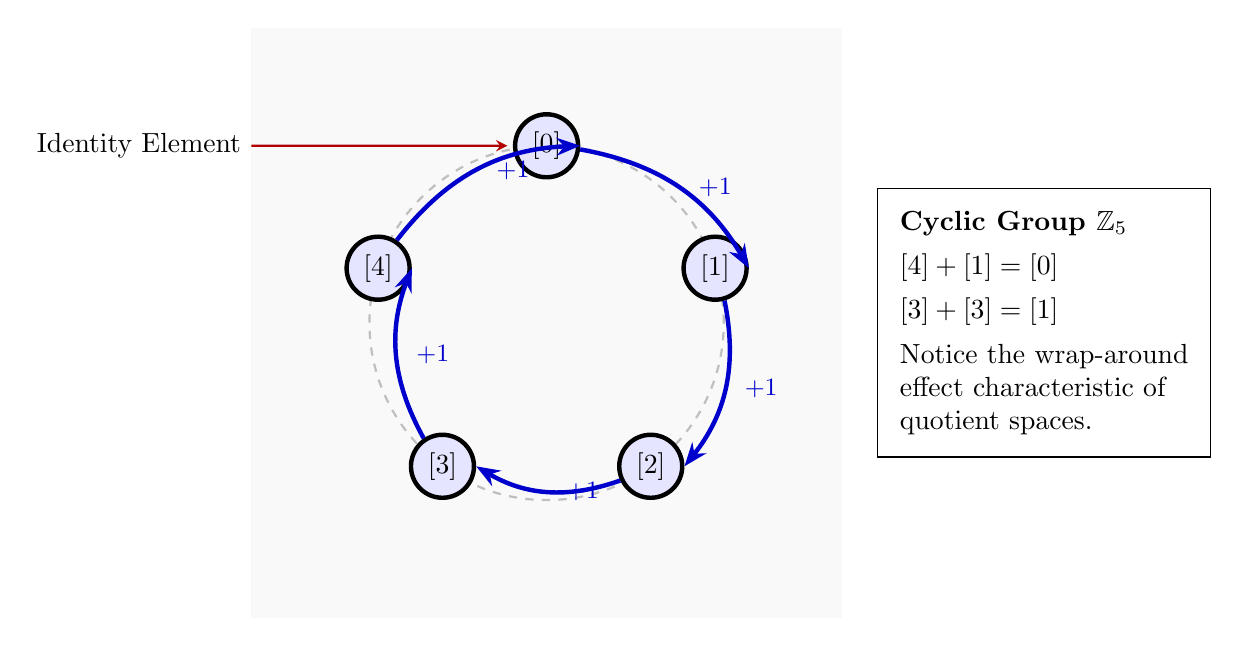
\begin{tikzpicture}[scale=1.5]
    % 1) Backgrounds
    \fill[gray!5] (-2.5,-2.5) rectangle (2.5,2.5);
    
    % 2) Grid/Axes (Not applicable for cycle graph, but we draw the main circular path)
    \draw[thick, dashed, gray!50] (0,0) circle (1.5cm);
    
    % 3) Primary plots (Nodes and transition arrows)
    \foreach \i/\label in {0/[0], 1/[1], 2/[2], 3/[3], 4/[4]} {
        % Calculate angle: 90 degrees is top, subtract 72 degrees for each step
        \pgfmathsetmacro{\angle}{90 - \i * 72}
        \node[circle, draw, ultra thick, fill=blue!10, minimum size=8mm, inner sep=2pt] (N\i) at (\angle:1.5) {$\displaystyle \label$};
    }
    
    % Draw arrows for +1 transitions
    \foreach \i in {0,1,2,3,4} {
        \pgfmathsetmacro{\next}{mod(\i+1,5)}
        \draw[-{Stealth[length=3mm]}, ultra thick, blue!80!black] (N\i) to[bend left=25] node[midway, right=3pt, font=\small] {$+1$} (N\next);
    }
    
    % 4) Node labels/text (Legend using Anchor Pivot Strategy)
    \node[align=left, draw, fill=white, inner sep=8pt, anchor=west] at (2.8, 0) {
        \textbf{Cyclic Group $\Z_5$}\\[4pt]
        $\displaystyle [4] + [1] = [0]$\\[4pt]
        $\displaystyle [3] + [3] = [1]$\\[4pt]
        Notice the wrap-around\\
        effect characteristic of\\
        quotient spaces.
    };
    
    % Off-axis callout
    \draw[->, >=stealth, shorten >=2pt, thick, red!70!black] (-2.5, 1.5) node[anchor=east, text=black] {Identity Element} -- (N0);
\end{tikzpicture}
\end{center}
\vspace{1em}

\subsection{Heuristics \& "Cheats"}
\begin{itemize}
    \item \textbf{Reduce Early, Reduce Often:} When calculating $[a^k]$ or $[a \cdot b]$, never compute the massive integer first. Reduce $a$ and $b$ modulo $n$ immediately, multiply, reduce again, and repeat.
    \item \textbf{Negative Numbers:} To quickly find the positive residue of a negative number $-x \pmod n$, simply add $n$ repeatedly until the number is positive. Example: $[-13] \pmod 8 \implies -13 + 8 = -5 \implies -5 + 8 = 3 \implies [3]$.
\end{itemize}

\subsection{Pitfalls \& Fallacies}
\begin{itemize}
    \item \textbf{The Cancellation Fallacy:} Assuming that if $[a][x] = [a][y]$, then $[x] = [y]$. This is \textbf{FALSE} in $\Z_n$ unless $\gcd(a, n) = 1$. For example, in $\Z_6$, $[2][2] = [2][5] = [4]$, but $[2] \neq [5]$.
    \item \textbf{Fractional Fallacy:} Never write fractions like $\frac{1}{2}$ in modular arithmetic. Division by $a$ is strictly defined as multiplication by the modular inverse of $a$, which only exists if $\gcd(a, n) = 1$.
\end{itemize}

\newpage
\section{Conceptual Synthesis and The "Big Picture"}

\subsection{Thematic Connections}
The central theme of this topic is \textbf{Quotient Structures and Isomorphisms}. By defining an equivalence relation on a set and operating on the equivalence classes, we compress an infinite space ($\Z$) into a finite space ($\Z_n$) while perfectly preserving the algebraic structure (addition and multiplication). This is the exact same thematic mechanism used in topology (gluing edges of a polygon to create a torus) and in measure theory (identifying functions that are equal "almost everywhere" to form $L^p$ spaces).

\subsection{Forward and Backward Links}
\begin{itemize}
    \item \textbf{Backward Links:} This topic relies heavily on the \textit{Division Algorithm} and \textit{Equivalence Relations} established in earlier chapters. It is the ultimate application of partitioning a set.
    \item \textbf{Forward Links:} $\Z_n$ is the bedrock of \textit{Abstract Algebra}. Understanding when $\Z_n$ has zero divisors leads directly to the definition of Integral Domains and Fields. Furthermore, the concept of a well-defined function on a quotient space is mandatory for understanding Lebesgue integration in advanced probability, where random variables are actually equivalence classes of measurable functions.
\end{itemize}

\section{Abstract Real-World Modeling (AI, ML, \& Quant Finance)}

\subsection{Concrete Scenarios}
\begin{enumerate}
    \item \textbf{Quantitative Finance (Monte Carlo Simulations):} Pricing complex exotic derivatives (like Asian or Barrier options) requires simulating millions of stochastic price paths. These simulations rely on Pseudo-Random Number Generators (PRNGs), the most fundamental of which is the Linear Congruential Generator operating entirely within $\Z_m$.
    \item \textbf{Cryptography (RSA Encryption):} Secure financial transactions rely on public-key cryptography. RSA operates on the multiplicative group of integers modulo $n$ (where $n = pq$ for large primes $p, q$), relying on the computational difficulty of factoring $n$ to invert modular exponentiation.
    \item \textbf{Computer Science (Hash Tables):} In algorithmic trading, order books must be updated in $O(1)$ time. Hash functions map massive order IDs to finite memory addresses using modular arithmetic ($h(x) = x \pmod m$), ensuring uniform distribution of data.
\end{enumerate}

\subsection{Rigorous Model Setup: Linear Congruential Generators in Option Pricing}
Suppose we are building a quantitative pricing engine for a European Call Option using Monte Carlo integration. We require a sequence of independent, identically distributed uniform random variables on $[0, 1)$. We model this using a Linear Congruential Generator (LCG) defined on the quotient ring $\Z_m$.

\textbf{State Space and Measure:}
Let the state space be the finite ring $\Z_m$. We define a deterministic transition function $f: \Z_m \to \Z_m$ such that:
\[
X_{k+1} = (a X_k + c) \pmod m
\]
where $a \in \Z_m$ is the multiplier, $c \in \Z_m$ is the increment, and $X_0 \in \Z_m$ is the seed. 

To map this to a probability space $(\Omega, \F, \Prob)$, we define the sample space $\Omega = [0, 1)$ equipped with the Borel $\sigma$-algebra $\mathcal{B}([0,1))$ and the Lebesgue measure $\lambda$. We construct a sequence of pseudo-random variables $U_k$:
\[
U_k = \frac{X_k}{m} \in [0, 1)
\]
\textbf{Optimization and Constraints:}
For the sequence $U_k$ to approximate the uniform measure $\lambda$ effectively (avoiding lattice structure flaws), the LCG must have a full period of $m$. By the Hull-Dobell Theorem, this requires specific number-theoretic constraints on our modular space:
1. $\gcd(c, m) = 1$.
2. $p \mid (a - 1)$ for all prime factors $p$ of $m$.
3. $4 \mid (a - 1)$ if $4 \mid m$.

Under these constraints, the expectation of the discounted payoff function $\Phi(S_T)$ under the risk-neutral measure $\mathbb{Q}$ can be approximated via the Law of Large Numbers:
\[
\E^{\mathbb{Q}}[e^{-rT} \Phi(S_T)] \approx \frac{1}{N} \sum_{k=1}^{N} e^{-rT} \Phi\left( S_0 \exp\left( \left(r - \frac{\sigma^2}{2}\right)T + \sigma \sqrt{T} \Phi^{-1}(U_k) \right) \right)
\]
where $\Phi^{-1}$ is the inverse CDF of the standard normal distribution, mapping our modular-generated uniform variables into Gaussian shocks for the stochastic differential equation $dS_t = r S_t dt + \sigma S_t dW_t$.

\newpage
\section{Common Variations and Untested Concepts}

A critical concept often tested in advanced courses, but missing from this specific homework set, is the existence of \textbf{Multiplicative Inverses} in $\Z_n$. 

\begin{theorem}[Existence of Modular Inverses]
An element $[a] \in \Z_n$ has a multiplicative inverse (an element $[x]$ such that $[a][x] = [1]$) if and only if $\gcd(a, n) = 1$.
\end{theorem}

\textbf{Worked Example / Proof:}
Prove that $[3]$ has a multiplicative inverse in $\Z_{10}$, but $[4]$ does not.

\textit{Proof:} 
For $[3] \in \Z_{10}$, we check $\gcd(3, 10) = 1$. By Bézout's Identity, there exist integers $x, y$ such that $3x + 10y = 1$. Using the Extended Euclidean Algorithm, we find $3(7) + 10(-2) = 1$. 
Taking this equation modulo 10 yields:
\[
3(7) \equiv 1 \pmod{10} \implies [3][7] = [1]
\]
Thus, $[7]$ is the multiplicative inverse of $[3]$.

For $[4] \in \Z_{10}$, $\gcd(4, 10) = 2 \neq 1$. Suppose for contradiction that an inverse $[x]$ exists, meaning $[4][x] = [1]$. This implies $4x \equiv 1 \pmod{10}$, or $4x - 10y = 1$ for some integer $y$. Factoring out a 2 gives $2(2x - 5y) = 1$. Since $x, y \in \Z$, $2x - 5y$ is an integer, implying that 2 divides 1, which is a contradiction. Thus, $[4]$ has no inverse.
\hfill $\blacksquare$

\section{Advanced Diagnostic Testing: "Find the Flaw"}

Below are five proofs containing subtle logical or mathematical flaws. Your task as the grader is to identify the error. The solutions are provided at the end.

\textbf{Problem 1:} Prove that if $ax \equiv ay \pmod n$, then $x \equiv y \pmod n$.
\textit{Flawed Proof:} We are given $ax \equiv ay \pmod n$. By the definition of congruence, this means $[ax] = [ay]$ in $\Z_n$. We can factor out the $[a]$ to get $[a][x] = [a][y]$. Dividing both sides of the equation by $[a]$ yields $[x] = [y]$, which means $x \equiv y \pmod n$. $\blacksquare$

\textbf{Problem 2:} Let $f: \Z_3 \to \Z_2$ be defined by $f([x]_3) = [x^2]_2$. Prove that $f$ is a well-defined function.
\textit{Flawed Proof:} Let $[a]_3 = [b]_3$. Then $a \equiv b \pmod 3$, so $a = b + 3k$ for some $k \in \Z$. We evaluate $f([a]_3) = [a^2]_2 = [(b+3k)^2]_2 = [b^2 + 6bk + 9k^2]_2$. Since $6bk$ is even, it is $0 \pmod 2$. Thus, $[b^2 + 9k^2]_2$. Since $9 \equiv 1 \pmod 2$, this is $[b^2 + k^2]_2$. If we choose $k$ to be even, $k^2 \equiv 0 \pmod 2$, leaving $[b^2]_2 = f([b]_3)$. Thus, the output is the same, and the function is well-defined. $\blacksquare$

\textbf{Problem 3:} Prove that for any integer $a$, $a^5 \equiv 1 \pmod 6$ if $\gcd(a, 6) = 1$.
\textit{Flawed Proof:} We wish to evaluate $a^{n-1} \pmod n$ where $n=6$. By Fermat's Little Theorem, for any integer $a$ coprime to $n$, we have $a^{n-1} \equiv 1 \pmod n$. Substituting $n=6$, we get $a^{6-1} = a^5 \equiv 1 \pmod 6$. $\blacksquare$

\textbf{Problem 4:} Solve the congruence $x^2 \equiv 1 \pmod 8$.
\textit{Flawed Proof:} We have $x^2 - 1 \equiv 0 \pmod 8$, which factors as $(x-1)(x+1) \equiv 0 \pmod 8$. For the product of two numbers to be zero, one of them must be zero. Thus, either $x-1 \equiv 0 \pmod 8 \implies x \equiv 1 \pmod 8$, or $x+1 \equiv 0 \pmod 8 \implies x \equiv 7 \pmod 8$. The only solutions are $x \in \{1, 7\}$. $\blacksquare$

\textbf{Problem 5:} Prove that $\Z_n$ has no zero divisors if $n$ is odd.
\textit{Flawed Proof:} Suppose $[a][b] = [0]$ in $\Z_n$. Then $n \mid ab$. Since $n$ is odd, it does not contain 2 as a prime factor. Therefore, $n$ cannot be split evenly between $a$ and $b$ in terms of powers of 2. Thus, $n$ must fully divide $a$ or fully divide $b$, meaning $[a]=[0]$ or $[b]=[0]$. $\blacksquare$

\vspace{1em}
\hrule
\vspace{1em}
\textbf{Solution Key (The Flaws):}
\begin{itemize}
    \item \textbf{Flaw 1:} The cancellation law (division) is invalid in $\Z_n$ unless $\gcd(a, n) = 1$. You cannot arbitrarily "divide by $[a]$" because $[a]$ might be a zero divisor and lack a multiplicative inverse.
    \item \textbf{Flaw 2:} The proof assumes we can "choose $k$ to be even". In proving well-definedness, the result must hold for \textit{all} valid representatives, meaning \textit{all} $k \in \Z$. If $k=1$, $f([0]_3) = [0]_2$, but $0 \equiv 3 \pmod 3$, and $f([3]_3) = [9]_2 = [1]_2$. Since $[0]_2 \neq [1]_2$, the function is actually NOT well-defined.
    \item \textbf{Flaw 3:} Fermat's Little Theorem strictly requires the modulus $n$ to be a \textit{prime} number. Since $6$ is composite, the theorem cannot be applied. (Euler's Totient Theorem must be used instead, and $\phi(6) = 2$, not 5).
    \item \textbf{Flaw 4:} The Zero Product Property ($ab=0 \implies a=0$ or $b=0$) only holds in integral domains. $\Z_8$ is not an integral domain. The numbers $x=3$ and $x=5$ are also valid solutions because $3^2 = 9 \equiv 1 \pmod 8$ and $5^2 = 25 \equiv 1 \pmod 8$.
    \item \textbf{Flaw 5:} The logical deduction "cannot be split evenly... thus $n$ must fully divide $a$" is nonsense. Consider $n=9$ (which is odd). Let $a=3$ and $b=3$. Then $n \mid ab$ ($9 \mid 9$), but $9 \nmid 3$. Odd composite numbers absolutely have zero divisors.
\end{itemize}

\end{document}